\documentclass[ignorenonframetext,]{beamer}
\usepackage{amssymb,amsmath}
\usepackage{ifxetex,ifluatex}
\usepackage{fixltx2e} % provides \textsubscript
\usepackage{tikz}
\usepackage{tikz-qtree}
\ifxetex
  \usepackage{fontspec,xltxtra,xunicode}
  \defaultfontfeatures{Mapping=tex-text,Scale=MatchLowercase}
\else
  \ifluatex
    \usepackage{fontspec}
    \defaultfontfeatures{Mapping=tex-text,Scale=MatchLowercase}
  \else
    \usepackage[utf8]{inputenc}
  \fi
\fi

% Comment these out if you don't want a slide with just the
% part/section/subsection/subsubsection title:
\AtBeginPart{
  \let\insertpartnumber\relax
  \let\partname\relax
  \frame{\partpage}
}
\AtBeginSection{
  \let\insertsectionnumber\relax
  \let\sectionname\relax
  \frame{\sectionpage}
}
\AtBeginSubsection{
  \let\insertsubsectionnumber\relax
  \let\subsectionname\relax
  \frame{\subsectionpage}
}

\setlength{\parindent}{0pt}
\setlength{\parskip}{6pt plus 2pt minus 1pt}
\setlength{\emergencystretch}{3em}  % prevent overfull lines
\setcounter{secnumdepth}{0}

\title{BA-PIEC International Economics}
\author{Instructer: David Jinkins}
\date{Date: Sept. 2, 2014}

\begin{document}
\frame{\titlepage}

\begin{frame}

\begin{itemize}
\itemsep1pt\parskip0pt\parsep0pt
\item
  Today

  \begin{itemize}
  \itemsep1pt\parskip0pt\parsep0pt
  \item
        Administrative stuff
  \item
        Why you should care about international economics
  \item
        Lightning couse overview
  \item
        Some facts about world trade
  \item
        Trade and gravity
  \end{itemize}
\end{itemize}

\end{frame}

\begin{frame}

\begin{itemize}
\itemsep1pt\parskip0pt\parsep0pt
\item
  Basic course structure:

  \begin{itemize}
  \itemsep1pt\parskip0pt\parsep0pt
  \item
    Weeks 1-4, trade
  \item
    Weeks 5-7, international finance
  \end{itemize}
\end{itemize}

\end{frame}

\begin{frame}

\begin{itemize}
\itemsep1pt\parskip0pt\parsep0pt
\item
  The textbook:

  \begin{itemize}
  \itemsep1pt\parskip0pt\parsep0pt
  \item
    International Economics: Theory and Policy, Krugman, Obstfeld, and
    Melitz, 10th edition.
  \item
    Two semesters recommended
    \begin{itemize}
        \item We are doing it in one quarter!
    \end{itemize}
  \item
    Online tutoring from textbook publisher 
    \begin{itemize}
        \item To access: pearsonmylabandmastering.com
        \item Use my course id:  jinkins85236
        \item Free subscription with new text book
        \item Not required, apparently helps in reviewing textbook 
    \end{itemize}
  \end{itemize}
\end{itemize}

\end{frame}

\begin{frame}

\begin{itemize}
\itemsep1pt\parskip0pt\parsep0pt
\item
    Class locations and times

  \begin{itemize}
  \itemsep1pt\parskip0pt\parsep0pt
  \item
    Tuesdays, SPs05 Lecture 11:40, 3 hrs
  \item
    Wednesdays, SPs05 Exercise 14:25, 2 hrs
  \item
    Tuesdays, SPs16 Lecture 8:55, 3 hrs
  \end{itemize}
  \item No exercise class this week!
\end{itemize}

\end{frame}

\begin{frame}

\begin{itemize}
\itemsep1pt\parskip0pt\parsep0pt
\item
  Course evaluation:

  \begin{itemize}
  \itemsep1pt\parskip0pt\parsep0pt
  \item
    23 October: A four-hour, closed-book written examination
  \item
    Based on

    \begin{itemize}
    \itemsep1pt\parskip0pt\parsep0pt
    \item
      Problem sets
    \item
      Lecture content
    \item
      Textbook
    \end{itemize}
  \item
    Everything from class, homework, or textbook is fair game
  \item
    Administrative questions? Tina Østergaard, toe.stu@cbs.dk
  \end{itemize}
\end{itemize}

\end{frame}

\begin{frame}

\begin{itemize}
\itemsep1pt\parskip0pt\parsep0pt
\item
  Email policy:

  \begin{itemize}
  \itemsep1pt\parskip0pt\parsep0pt
  \item
    Don't send me emails -(unless absolutely necessary)
  \item
    Instead\ldots
  \end{itemize}
\end{itemize}

\end{frame}

\begin{frame}

\begin{itemize}
\itemsep1pt\parskip0pt\parsep0pt
\item
  Course wiki:

  \begin{itemize}
  \itemsep1pt\parskip0pt\parsep0pt
  \item
    link at davidjinkins.com
  \item
    other class-related stuff there
  \item
    it's my first time with wiki
  \end{itemize}
\end{itemize}

\end{frame}


\begin{frame}

\begin{itemize}
\itemsep1pt\parskip0pt\parsep0pt
\item
    End administrative section
\end{itemize}

\end{frame}


\begin{frame}

    \begin{itemize}
    \itemsep1pt\parskip0pt\parsep0pt
        \item
        Section 2: Why should you care about international economics?
        \begin{itemize}
        \itemsep1pt\parskip0pt\parsep0pt
            \item Personally: Denmark is a small, open economy
            \item Politically: News articles often incomplete
            \item Intellectually: Many puzzles, some without explanation
        \end{itemize}
    \end{itemize}

\end{frame}

\begin{frame}

    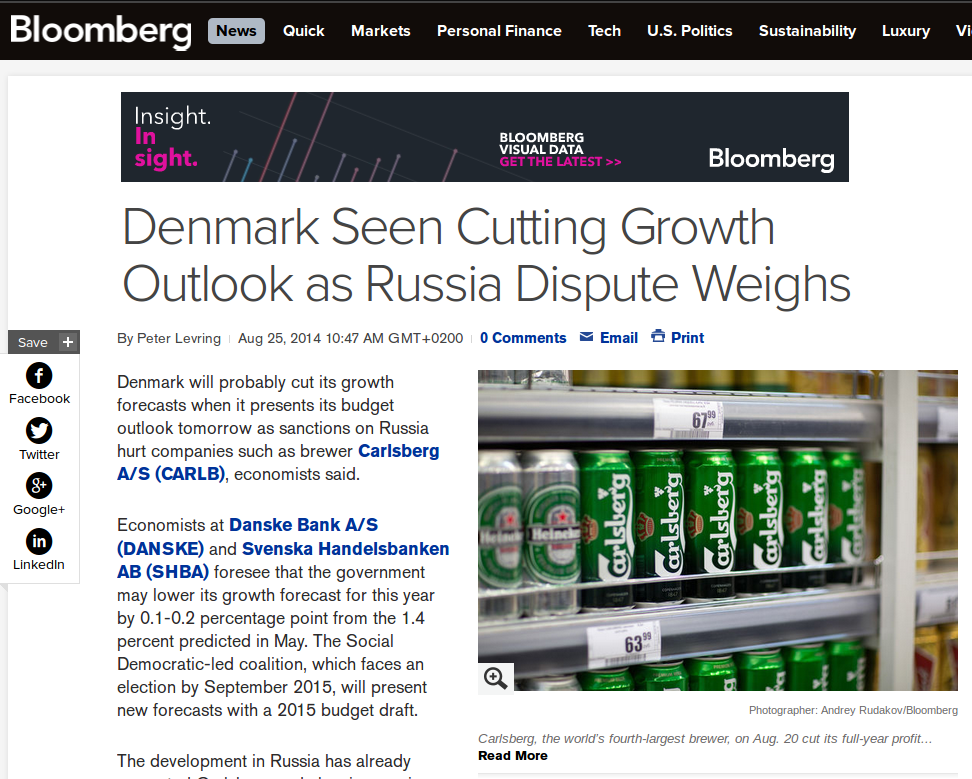
\includegraphics[scale=0.3]{carlsberg_political.png}

    {\tiny Source: http://www.bloomberg.com/news/2014-08-24/denmark-seen-cutting-growth-outlook-as-russia-dispute-weighs.html }

\end{frame}

\begin{frame}

    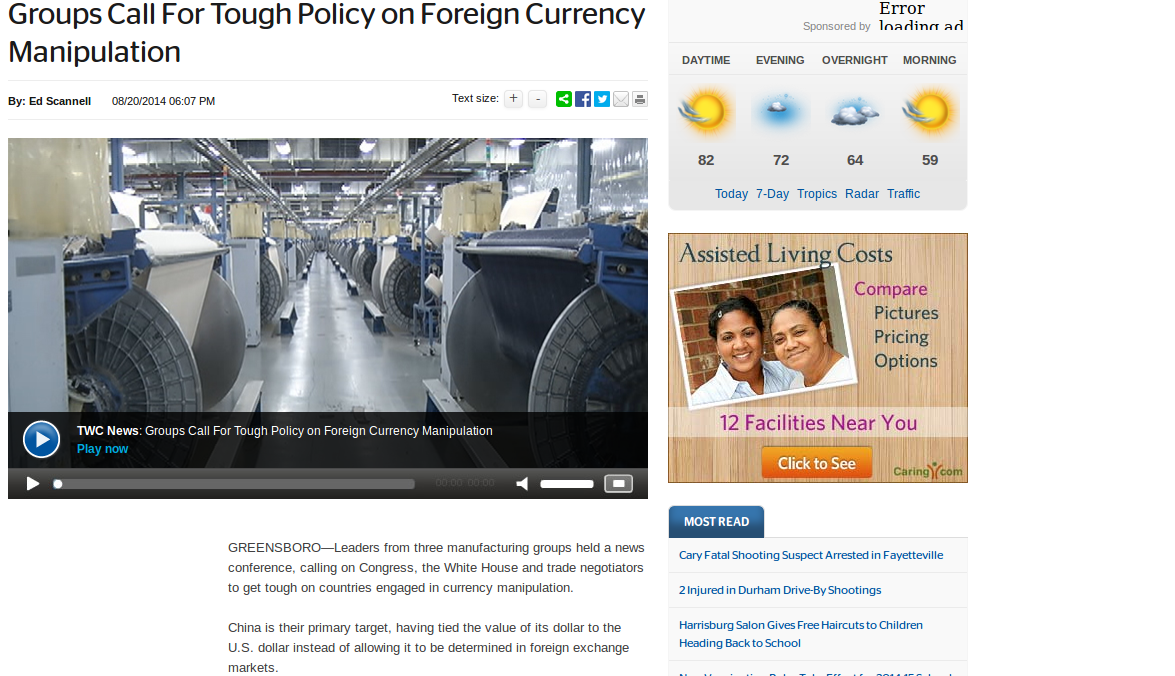
\includegraphics[scale=0.3]{currency_manipulation.png}

    {\tiny Source: http://triadnc.twcnews.com/content/news/711005/groups-call-for-tough-policy-on-foreign-currency-manipulation/}

\end{frame}

\begin{frame}

    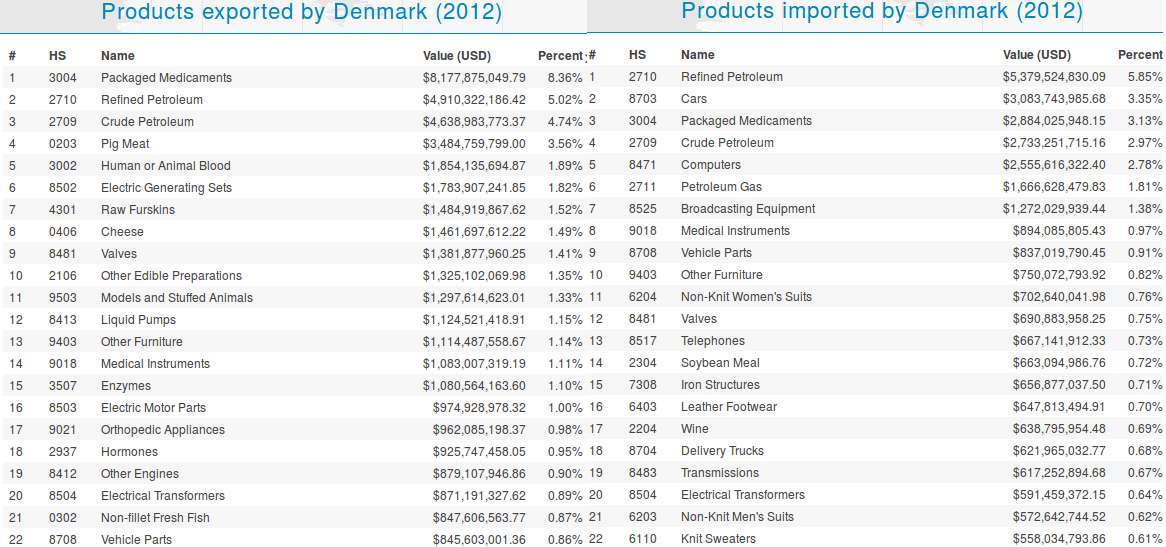
\includegraphics[scale=0.28]{Denmark_disaggregated_trade.png}
    
    {\tiny Source: http://atlas.media.mit.edu/explore/tree\_map/hs/import/dnk/all/show/2012/}

\end{frame}

\begin{frame}

    \begin{itemize}
        \item Section 3: Lightning overview
    \end{itemize}

\end{frame}

\begin{frame}{Why International Economics?}
\end{frame}


\begin{frame}{Why International Economics?}

    \begin{itemize}
        \item Not easy to move capital and especially labor across borders
        \item Many countries have different currencies
        \item Countries have different government policies 
        \item Hard to enforce contracts internationally
        \item Countries may be better or worse at making different products 
        \begin{itemize}
            \item Climate for agricuture
            \item More generally, technology
        \end{itemize}
        \item Culture, language, tastes, etc are more likely to differ
        \item Last but not least:
        \begin{itemize}
            \item Because of tariff collection, excellent data on shipments between countries
        \end{itemize}
    \end{itemize}
\end{frame}
    
\begin{frame}

\begin{tikzpicture}
\tikzset{scale=0.75,grow'=right,level distance=70pt}
\tikzset{execute at begin node=\strut}
\tikzset{every tree node/.style={anchor=base west}}

\Tree   [.Int\ Econ                     [.Trade     [.Theory    [.Comparative\ advantage ]
                                                                [.Factor\ endowments ]
                                                                [.Specific\ factors ]
                                                                [.Scale\ economies ]
                                                                [.Standard\ model ] ]
                                                    [.Policy    [.Policy\ instruments ]
                                                                [.Political\ economy ] ] ]
                                        [.Finance   [.Theory    [.Terminology\ and\ principles ]
                                                                [.Long-run\ exchange\ rates ] ]
                                                    [.Policy    [.Short-run\ exchange\ rates ]
                                                                [.Coordination\ and\ Currency\ unions ] ] ] ]
\end{tikzpicture}

\end{frame}

\begin{frame}{Comparative Advantage}

    \begin{itemize}
        \item A country gains from trade, even if it is better at everything than all other countries
        \item {\footnotesize\emph{To a trained economist, the basic [comparative advantage] model seems almost trivial. Two goods, two countries, one productive factor, perfect competition: what could be simpler? Indeed, one of the fierce joys of being an international trade economist is that so many seemingly sophisticated tracts can be revealed as nonsense, so many self-important men unmasked as poseurs, using such a minimalist framework. And yet if one tries to explain the basic model to a non-economist, it soon becomes clear that it really isn't that simple after all. -Paul Krugman http://web.mit.edu/krugman/www/ricardo.htm}}
    \end{itemize}

\end{frame}

\begin{frame}{Factor endowments}

    \begin{itemize}
        \item Obvious idea: China lots of labor $\implies$ textiles, Denmark lots of capital $\implies$ medical machinery
        \item For a long time, this was \emph{the} economic trade model (Heckscher-Ohlin)
        \item Question: How do trade patterns  change in response to technological changes?
    \end{itemize}

\end{frame}

\begin{frame}{Specific factors}

    \begin{itemize}
        \item Lesson of early trade models: trade is great! 
        \item Great for who -- who is hurt by trade?
    \end{itemize}

\end{frame}

\begin{frame}{Specific factors}

    
\includegraphics[scale=0.3]{jobs_to_london.png}

\end{frame}

\begin{frame}{Scale economies}

    \begin{itemize}
        \item Specialization: Theme of introductory microecon.
        \item Decreasing marginal costs of production.
        \item Historical accident and the location of Silicon Valley.
        \item Multiple equilibria in trade models.
    \end{itemize}

\end{frame}

\begin{frame}{Policy instruments}

    \begin{itemize}
        \item tariffs, quotas, subsidies
        \item product specifications
    \end{itemize}

\end{frame}

\begin{frame}{Political economy}

    \begin{itemize}
        \item Can trade policy be good for a country?
        \item Is trade policy good for a country?
        \item How is trade policy made
    \end{itemize}

\end{frame}

\begin{frame}{Finance: terms and principles}

    \begin{itemize}
        \item Basic issue:
        \begin{itemize}
            \item Exporters paid in dollars
            \item Costs are in kroner
        \end{itemize}
        \item Exchange rates are critical
        \item Terminology: balance of accounts, trade deficit, etc. 
        \item More generally, international risk sharing
    \end{itemize}

\end{frame}

\begin{frame}{Exchange rates}

    \begin{itemize}
        \item What determines exchange rates in the long-run.  PPP?
        \item Short run: Is China a currency manipulator?
    \end{itemize}

\end{frame}

\begin{frame}{Currency Unions}

    \begin{itemize}
        \item Eliminate exchange rate uncertainty
        \item Policy coordination critical
    \end{itemize}

\end{frame}

\begin{frame}
    Section 4: Facts about international trade
\end{frame}

\begin{frame}

    \begin{itemize}
        \item What do countries trade:
        \begin{itemize}
            \item Agricultural produce
            \item Primary goods
            \item Manufactures
            \item Services
        \end{itemize}
        \item Composition of trade has changed over time
        \item Manufactures as a fraction of non-service trade
    \end{itemize}
    
    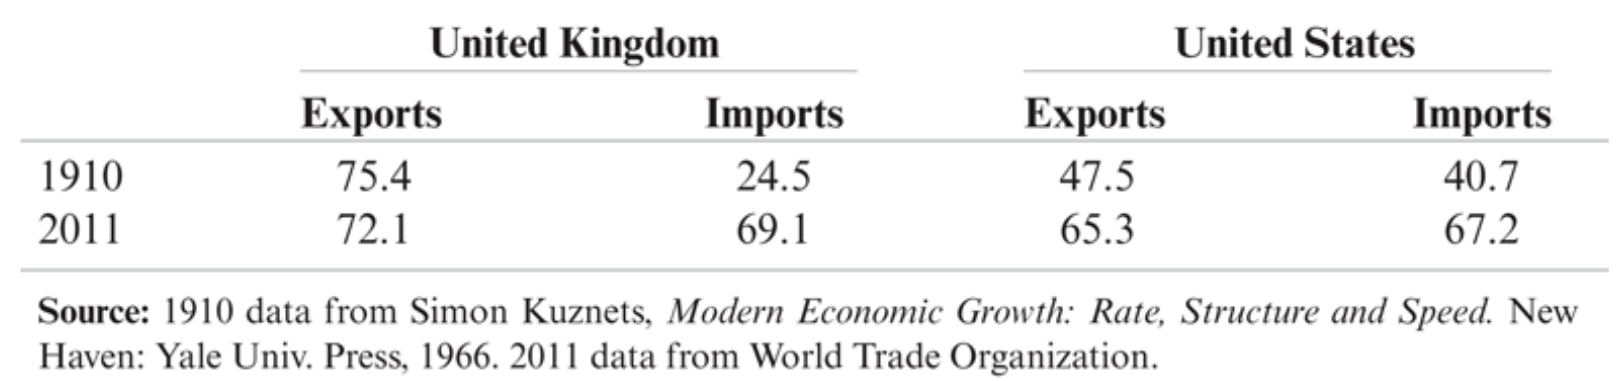
\includegraphics[scale=0.20]{us_uk_merchandise_trade.png}

\end{frame}

\begin{frame}

    \begin{itemize}
        \item Developing countries trade composition 
    \end{itemize}
    
    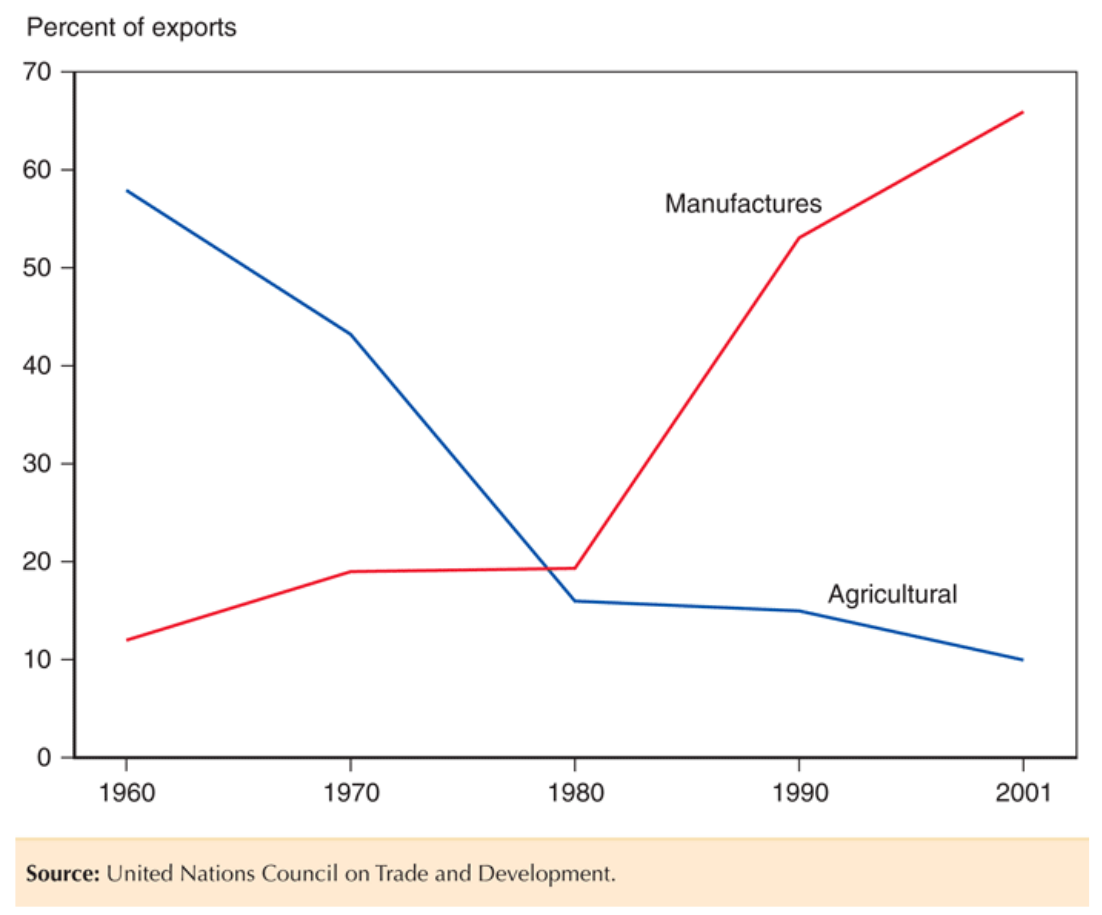
\includegraphics[scale=0.20]{developing_country_comp_adv.png}

\end{frame}

\begin{frame}

    \begin{itemize}
        \itemsep1pt\parskip0pt\parsep0pt
        \item `` In the early 21st century, nations are more closely linked than ever before through trade in goods and services\dots''
    \end{itemize}
   
    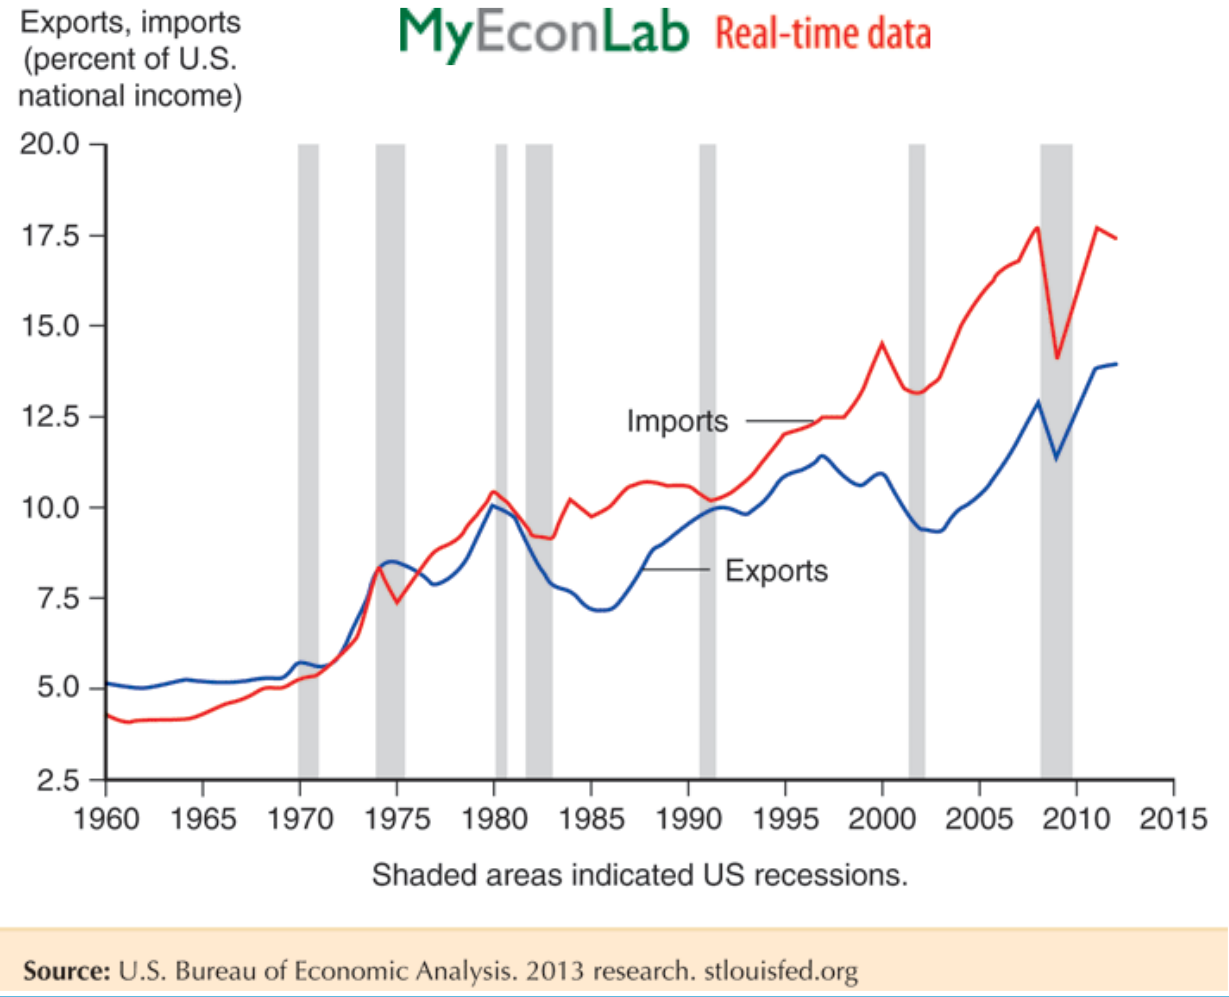
\includegraphics[scale=0.25]{figure1-1.png}

\end{frame}
    
\begin{frame}

    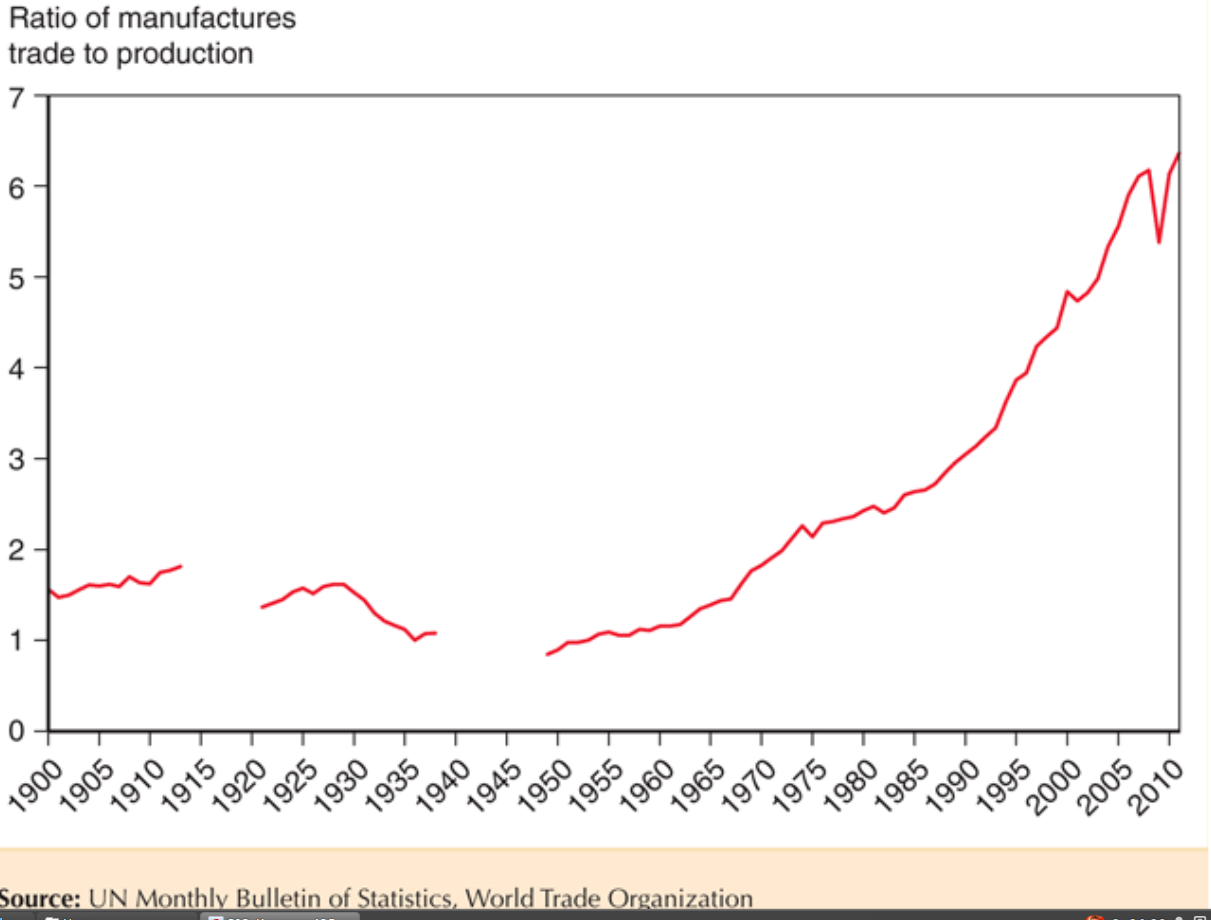
\includegraphics[scale=0.25]{Text_fig_2_5.png}

\end{frame}

\begin{frame}

    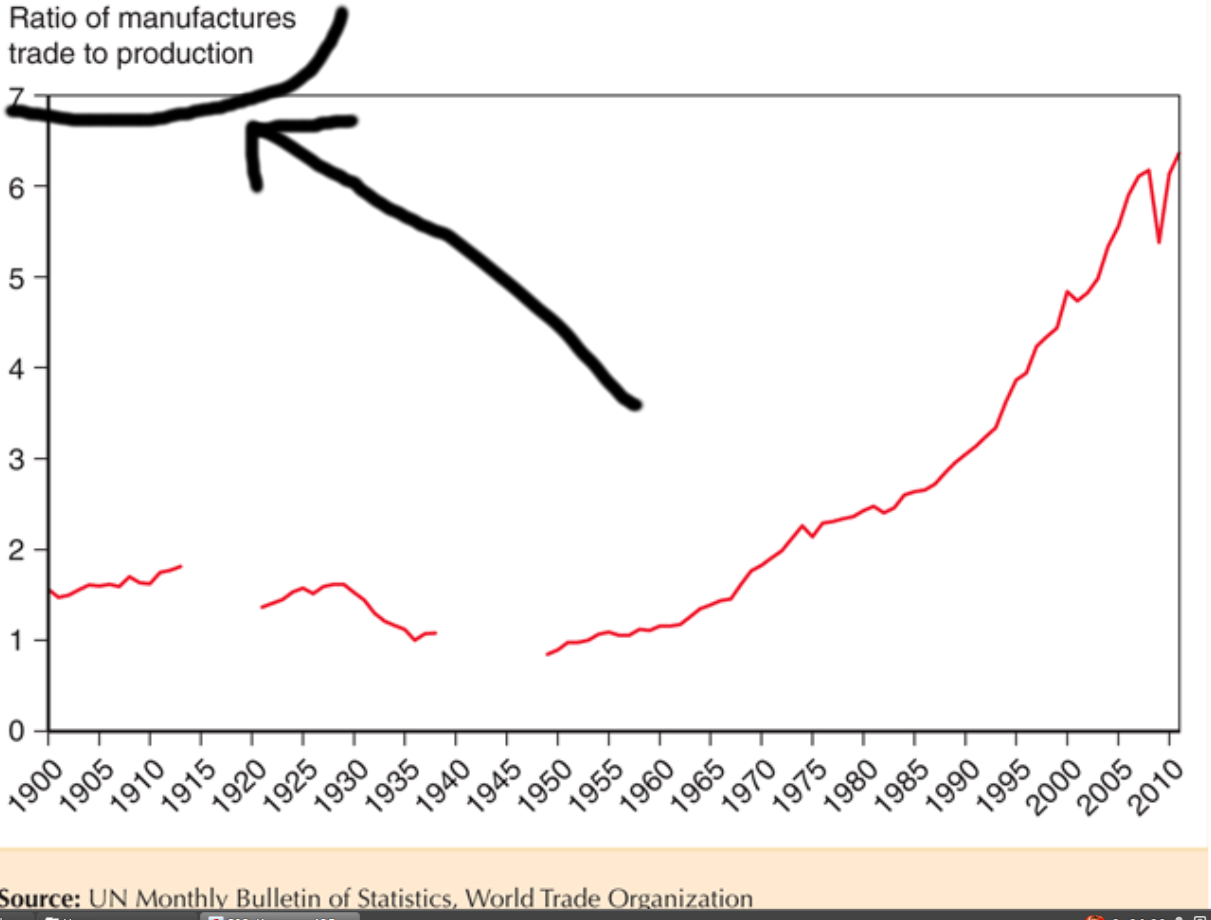
\includegraphics[scale=0.25]{Text_fig_2_5_tricky.png}

\end{frame}

\begin{frame}

    \begin{itemize}
        \itemsep1pt\parskip0pt\parsep0pt
        \item true, but\dots
    \end{itemize}
   
    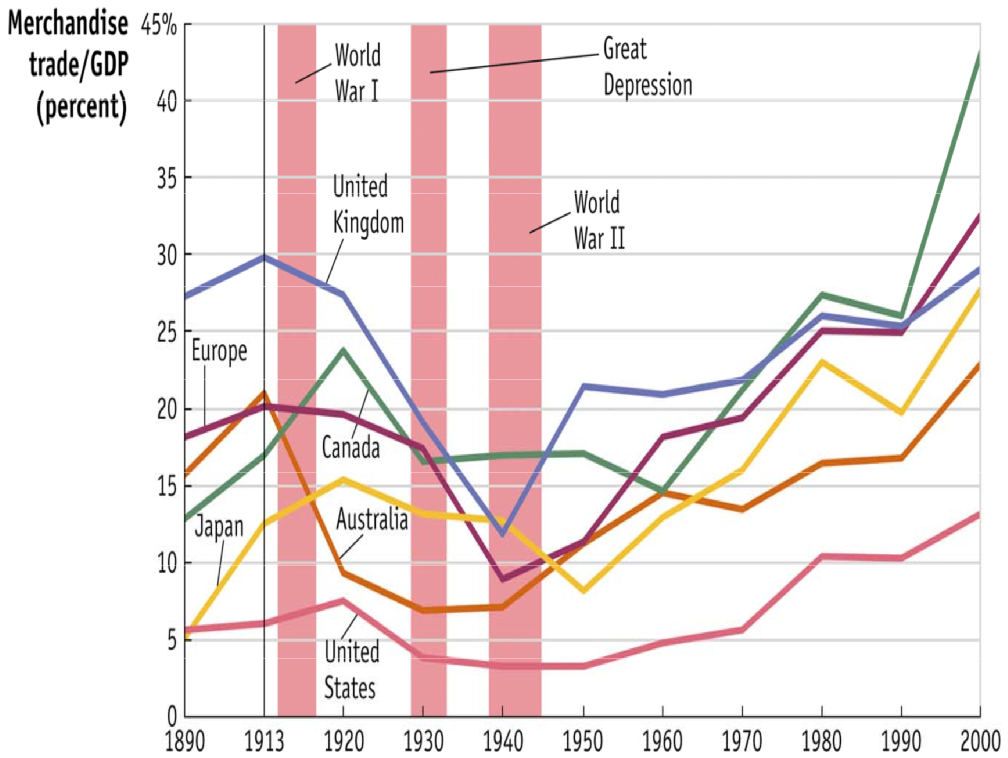
\includegraphics[scale=0.25]{trade_to_gdp_historical.png}

    {\tiny Source: Feenstra (1998)}

\end{frame}

\begin{frame}

    \begin{itemize}
        \item Service trade: Scary, because that is what developed countries do
        \item Labor force by sector (ag/manuf/service)
    \end{itemize}
    
    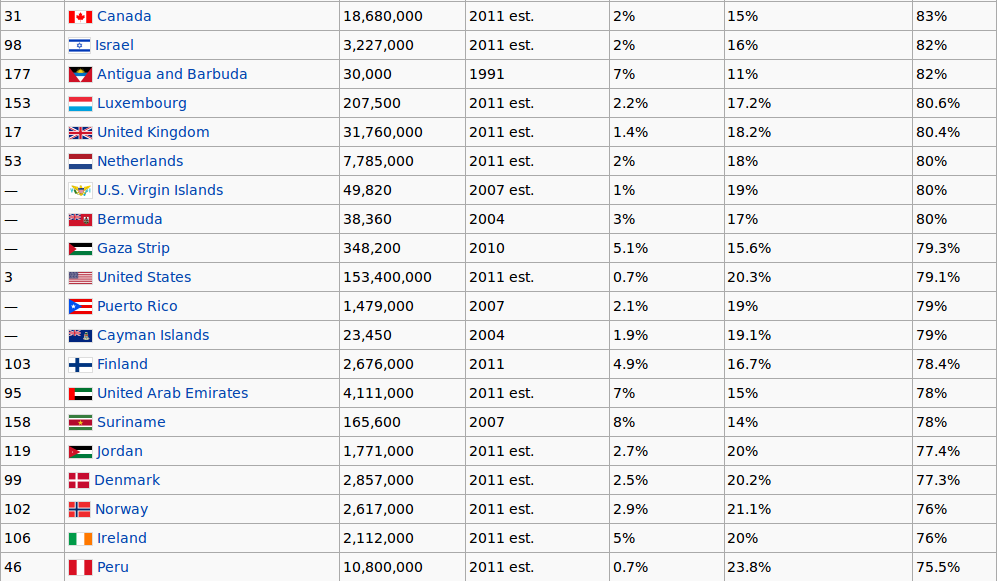
\includegraphics[scale=0.30]{sector_comp_of_labor_force.png}

    {\tiny Source: http://en.wikipedia.org/wiki/List\_of\_countries\_by\_sector\_composition\_of\_the\_labor\_force}

\end{frame}

\begin{frame}

   \begin{itemize}
        \item But many service jobs are 'non-tradable'
    \end{itemize}

    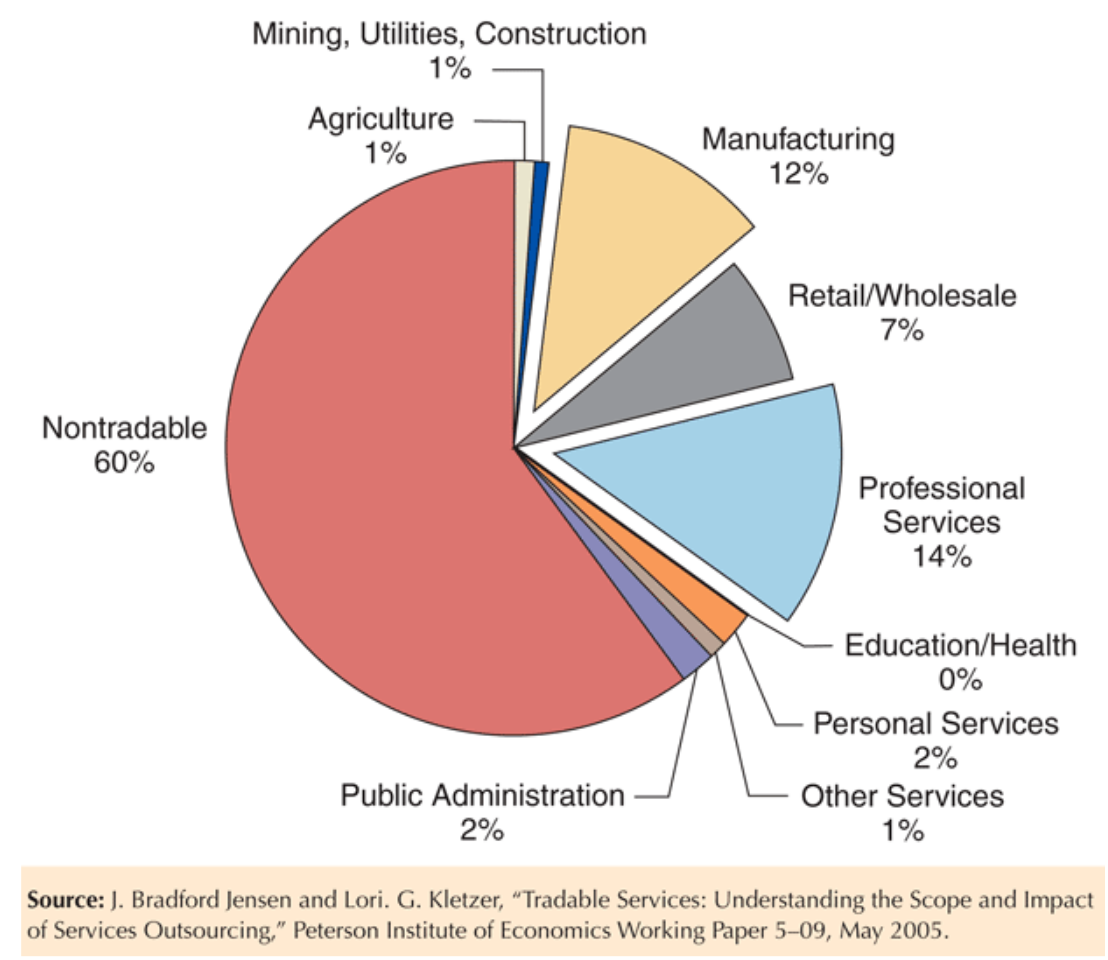
\includegraphics[scale=0.20]{tradable_services.png}

\end{frame}

\begin{frame}

   \begin{itemize}
        \item But many service jobs are 'non-tradable'
    \end{itemize}

    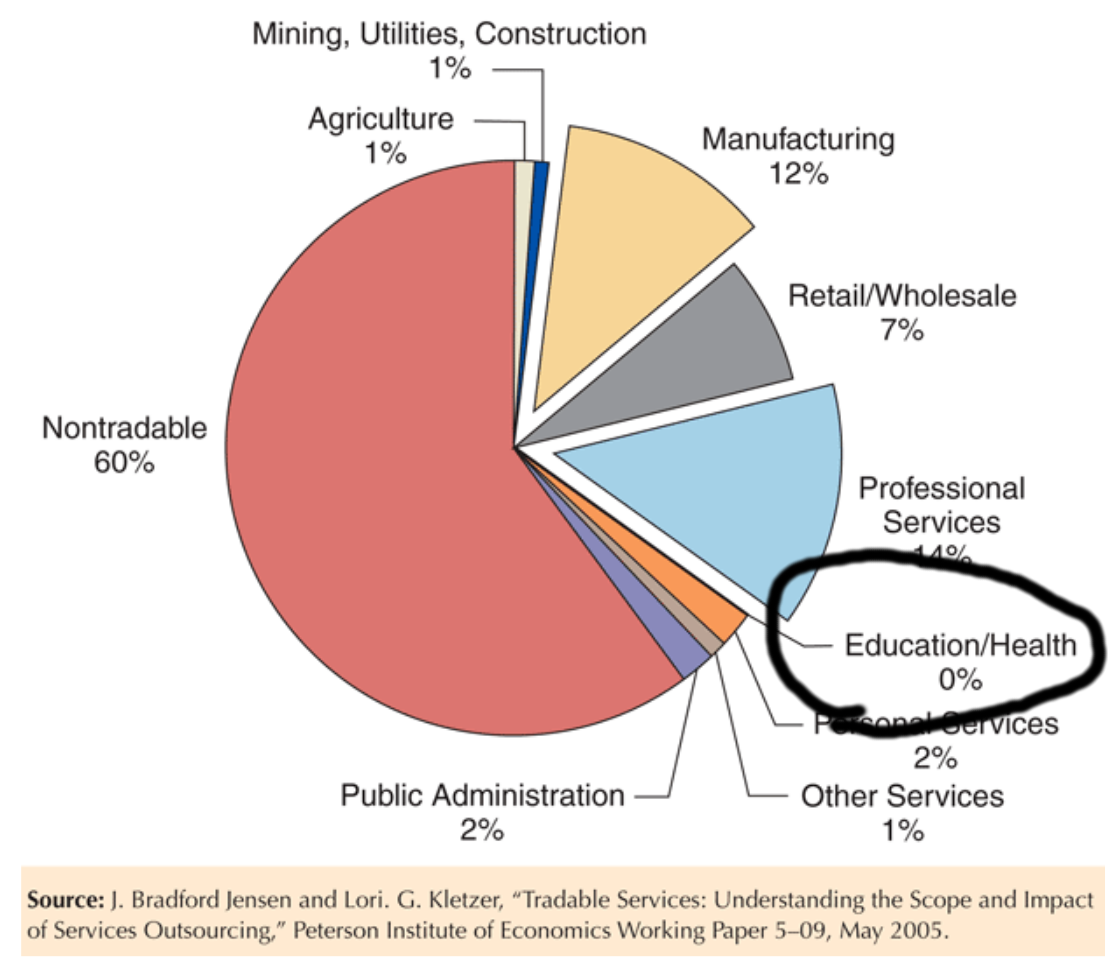
\includegraphics[scale=0.20]{tradable_services_yikes.png}

\end{frame}

\begin{frame}

    \begin{itemize}
        \item Section 5: Gravity and Trade
    \end{itemize}

\end{frame}

\begin{frame}
    
    \begin{itemize}
        \item Gravity equation (gravity):
        \begin{equation*}
            F_{ij} = g \frac{M_i M_j}{d_{ij}^2}
        \end{equation*}
        \item Gravity equation (trade):
        \begin{equation*}
            X_{ij} = g \frac{\mbox{GDP}_i \mbox{GDP}_j}{d_{ij}^\theta}
        \end{equation*}
        \item typically $\theta \approx 1$
        \item Empirical fact first observed by Tinbergen in 1960's.
    \end{itemize}

\end{frame}

\begin{frame}
   
    \begin{itemize}
        \item Numerator only
        \begin{equation*}
            T^*_{ij} = \mbox{GDP}_i \mbox{GDP}_j
        \end{equation*}
        \item Larger countries export more to all locations
        \item Larger countries import more from all locations
    \end{itemize}

\end{frame}

\begin{frame}
   
    \begin{itemize}
        \item Numerator only
    \end{itemize}
    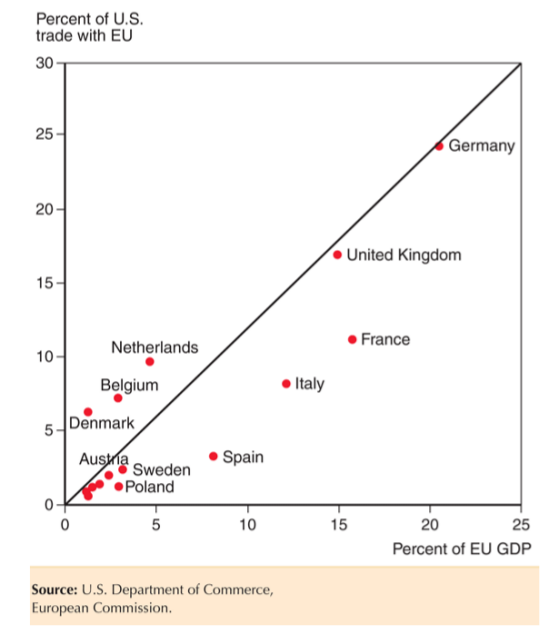
\includegraphics[scale=0.40]{gravity_numerator_fit.png}

\end{frame}

\begin{frame}

    \begin{itemize}
        \item Numerator only
    \end{itemize}
    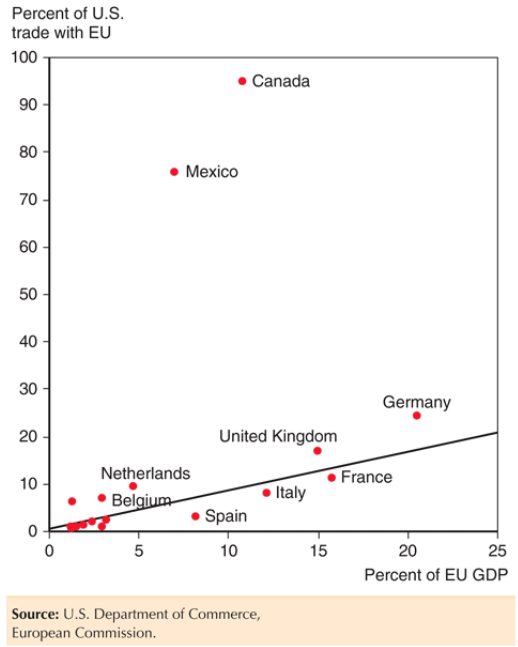
\includegraphics[scale=0.40]{gravity_numerator_fit_nafta.png}

\end{frame}

\begin{frame}{Missing trade}

    \begin{itemize}
        \item Distance extremely important for trade
        \item Doubling distance reduces trade by half
        \item Transport costs?
        \item Scale very little with distance
    \end{itemize}

\end{frame}

\begin{frame}{Missing trade}

    \begin{itemize}
        \item Physical distance a proxy:
        \item Nearby countries have:
        \begin{itemize}
            \item Similar Language
            \item Cultural Affinity
            \item Continguity 
        \end{itemize}
        \item Even so, puzzling how little countries trade
    \end{itemize}

\end{frame}

\begin{frame}{Missing trade}
    
    \begin{itemize}
        \item Canada has no tariffs with the United States
        \item Quite easy to cross the border
        \item ex: cross-border shopping
    \end{itemize}

\end{frame}

\begin{frame}{Missing trade}
    
    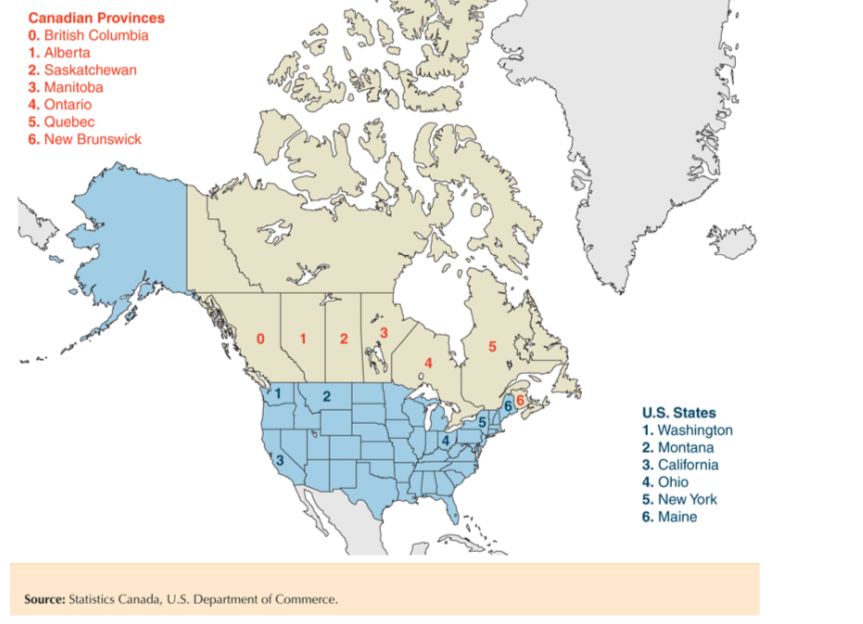
\includegraphics[scale=0.35]{canada_map.png}

\end{frame}

\begin{frame}{Missing trade}

    Trade with British Colombia, 2009 
    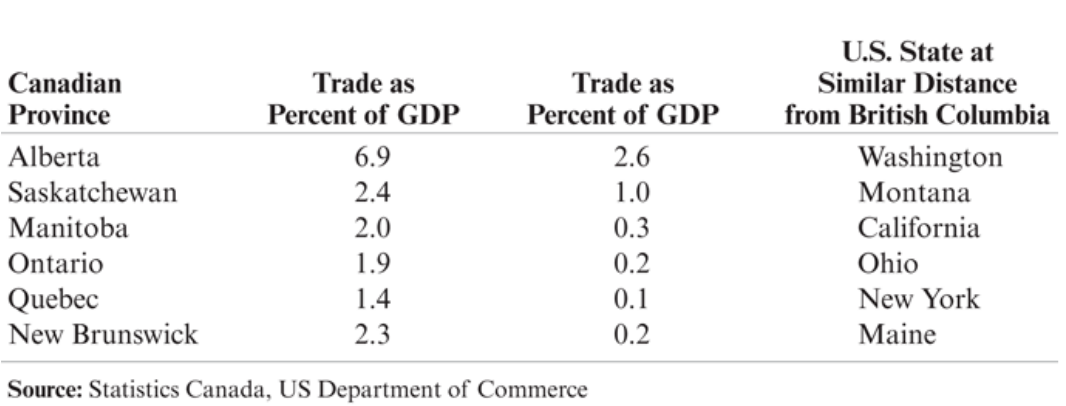
\includegraphics[scale=0.30]{canada_us_trade.png}

    Border effect same as 2500-4000 km of distance!

\end{frame}

\begin{frame}{Estimating Gravity}
    Gravity equation:
        \begin{equation*}
            X_{ij} = g \frac{\mbox{GDP}_i \mbox{GDP}_j}{d_{ij}^\theta}
        \end{equation*}
    Logs:
        \begin{equation*}
            \ln(X_{ij}) - \ln(\mbox{GDP}_i) - \ln(\mbox{GDP}_j) = \ln (g) + \theta \ln (d_{ij}) + \epsilon_{ij}
        \end{equation*}
\end{frame}

\begin{frame}

    Question: Does Denmark have more trade with UK or the United States?

    Why?

\end{frame}

\begin{frame}

    \begin{itemize}
        \item UK GDP 2.5 trillion USD
        \item US GDP 15 trillion USD
    \end{itemize}

    \begin{itemize}
        \item Pop. weighted UK-DK distance 1000 km
        \item Pop. weighted US-DK distance 7500 km 
    \end{itemize}

\end{frame}

\begin{frame}

    \begin{itemize}
        \item 2012 DK-UK exports 9 billion USD
        \item 2012 DK-USA exports 7.5 billion USD
    \end{itemize}

\end{frame}

\begin{frame}{Summary}

  \begin{itemize}
  \itemsep1pt\parskip0pt\parsep0pt
  \item Why you should care about international economics
        \begin{itemize}
            \item Denmark is a small open economy
            \item Poor media understanding of trade 
            \item Many puzzles, some not solved 
        \end{itemize}
  \item Lightning course overview
  \item Some facts about world trade
        \begin{itemize}
            \item More trade in manufactures, less agriculture over time 
            \item Trade share of gdp is growing 
            \item Service trade not so alarming 
        \end{itemize}
  \item Trade and gravity
        \begin{itemize}
            \item Trade closely follows a gravity specification
            \item Distance effect very strong, still a puzzle
        \end{itemize}
  \end{itemize}

\end{frame}

\begin{frame}

    \begin{itemize}
        \item Next time, the Ricardian (comparative advantage) model
        \begin{itemize}
            \item Countries trade due to technology differences
            \item There are always gains from trade, even for a country better at everything!
            \item A deeply counter-intuitive idea
        \end{itemize}
    \end{itemize}

\end{frame}

\end{document}


